% ===== 1. Introduction =====
\section{1. Introduction}\label{introduction}

\begin{figure}[t]
\centering
\pandocbounded{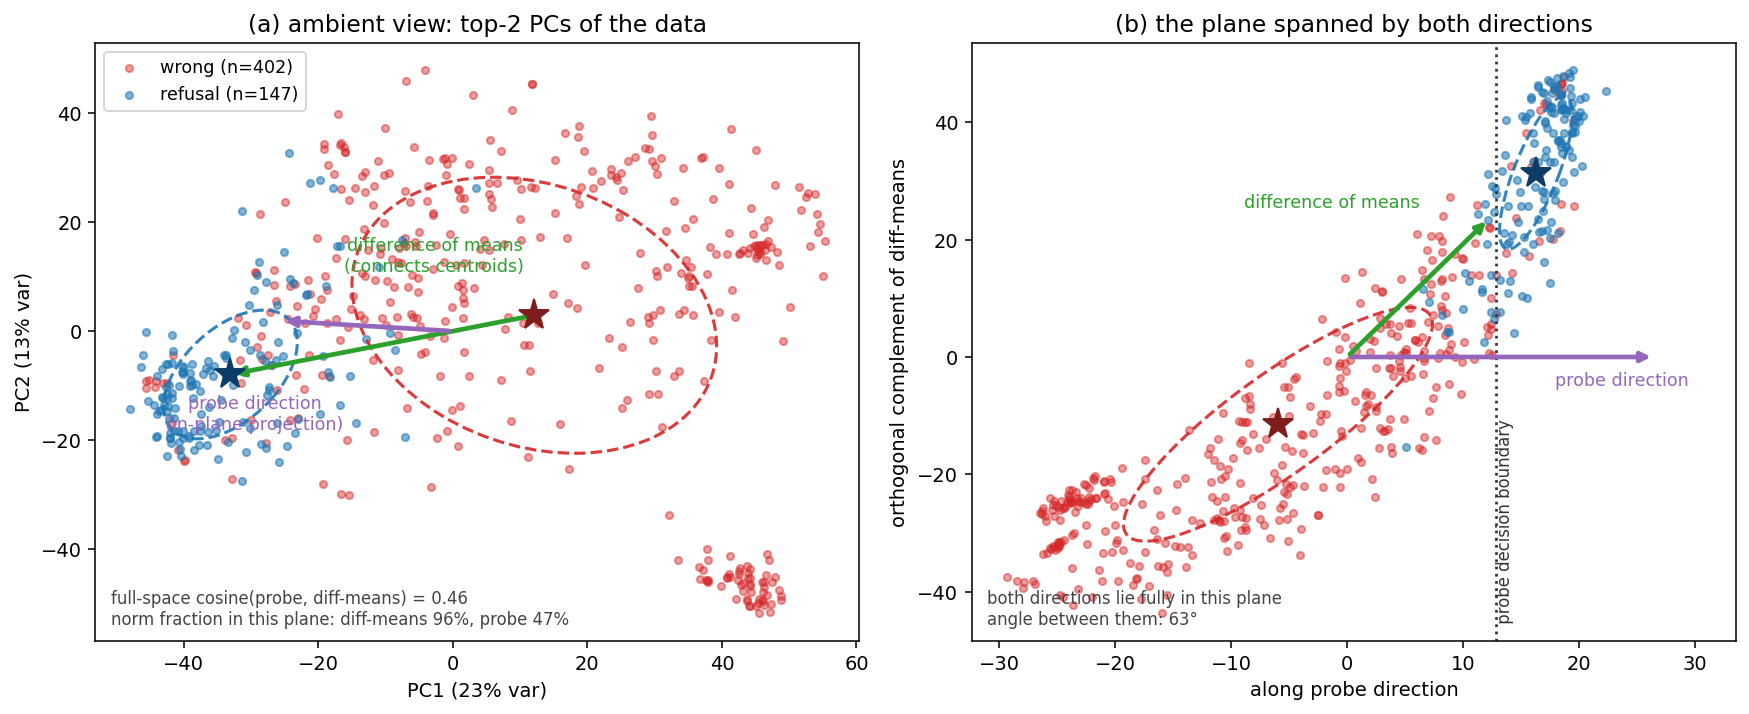
\includegraphics[keepaspectratio,alt={Two recoveries of ``the'' refusal
  direction (layer-28 refusal+wrong states, n=549; stars: class centroids; dashed curves:
  per-class 1\textbackslash sigma covariance ellipses). (a) Ambient view, top two
  principal components of the data: the class-mean difference (green) connects the
  centroids and lies almost entirely (96\textbackslash\% of its norm) in this top-variance
  plane; the probe direction (purple, in-plane projection) keeps only 47\textbackslash\%
  of its norm here. (b) The plane spanned by the two directions themselves, in which both
  lie fully: the angle between them is 63\^{}\textbackslash circ (full-space cosine 0.46).
  The refusal cluster separates along an oblique axis between the two arrows, and the
  wrong class's covariance ellipse is elongated along the same oblique axis: the centroid
  connector rides that high-variance content spread, while the probe direction is the axis
  whose marginal separates the classes item by item (its x-marginal here is, up to an
  affine map, the score histograms of Appendix D.4). The dotted vertical line is the probe's
  decision boundary, which is exact in this panel: the separating hyperplane's normal is
  the probe direction itself, so the boundary intersects this plane perpendicular to the
  x-axis.},width=0.9\linewidth]{figures/qwen3_1_7b/direction_geometry.png}}
\caption{Two recoveries of ``the'' refusal direction (layer-28
refusal+wrong states, \(n=549\); stars: class centroids; dashed curves:
per-class \(1\sigma\) covariance ellipses). \textbf{(a)} Ambient view,
top two principal components: the class-mean difference (green) connects
the centroids and lies almost entirely in this top-variance plane; the
probe direction (purple, in-plane projection) does not. \textbf{(b)} The
plane spanned by the two directions, in which both lie fully: the angle
between them is \(63^\circ\). The wrong class's covariance ellipse is
elongated along the same oblique axis the centroid connector rides,
while the probe direction is the axis whose marginal separates the
classes item by item (score histograms in Figure
\ref{fig:score-hist}). The dotted vertical line is the probe's decision
boundary, exact in this panel because the hyperplane normal is the probe
direction itself.}\label{fig:geometry}
\end{figure}

Confabulation is pattern-based reconstruction the model does not recognize as wrong, 
a term that expresses the nature of language-model (LM) answers better than ``hallucination'', which implies a false perception \citep{smith2023confabulation, farquhar2024semantic}. 
When a small LM (SLM) is asked a factual question about
something it does not know, it has a \emph{choice} to refuse or answer anyway.
A fraction of those answers happen to be correct; the rest are
confabulations: fluent, confident, and wrong.
Can we read that \emph{choice} off the
hidden state, and steer it? \citet{alain2017probes} introduced diagnostic linear classifiers, or
\emph{probes}, to evaluate what a hidden state encodes. \citet{kadavath2022know}
argued that LLMs ``mostly know what they know,'' and a correctness-probing
literature followed
\citep{azaria2023internal, marks2024geometry, orgad2024show, kossen2024semantic}, fitting probes to predict
whether an answer will be right and reporting accuracies in the \(80\)--\(90\%\) range.
High probe accuracy is not by itself evidence that the hidden state
knows anything. In adjacent settings, recent work traces above-chance
accuracy to the prompt rather than the model's internal state:
introspection \citep{singh2026introspect} and reasoning mode
\citep{sahoo2026linear}. A confabulation probe faces the same question.
Does it read the model's state, or the question?

Controls that separate hidden-state signal from what the prompt alone
predicts remain rare in the correctness-probing literature, where
time-sensitive question sets routinely conflate ``post-cutoff'' with
``model doesn't know.'' Refusal steering by a single direction has been shown for safety refusal \citep{arditi2024refusal}.
\citet{wollschlager2025geometry} showed that safety refusal can be steered by a set of directions. 
For knowledge-based refusals, \citet{ferrando2025entity} found that features corresponding to known entities suppress refusals on Gemma 2. 
\citet{lindsey2025biology} confirmed this for Haiku 3.5 and further investigated the multi-step mechanics triggered by these features.
I ask whether a single direction can convert most confabulations into refusals for facts the model did not learn.

I map the geometry of this decision with the probes, a sparse
autoencoder, and direct optimization of intervention direction.
To test whether steering along the recovered directions turns
confabulations into refusals I introduce \textbf{ConfabQA}, a probing benchmark of 4 domains
\(\times\) 3 categories (well-known pre-cutoff, \emph{obscure}
pre-cutoff, post-cutoff). The obscure category, items whose answers were likely in the training data but which the model is expected to fail, populates
the cell standard pre-vs-post-cutoff designs leave empty, breaking the
cutoff/correctness confound. ConfabQA, plus 800-item samples of PopQA
\citep{mallen2023popqa} and TriviaQA \citep{joshi2017triviaqa}, run through three
instruction-tuned models in the \(1.7\)--\(3\)B range (Qwen3-1.7B,
Gemma 2 2B, Llama 3.2 3B) with Qwen3-4B as a within-family scaling
control. Every probe is scored against both the majority and stricter question-text baselines to decide whether the
hidden state contributed anything.

\textbf{Findings}

\begin{enumerate}
\def\labelenumi{\arabic{enumi}.}
\item
  \emph{Refusal vs.~confabulation is a model-internal feature:} On the
  wrong+refusal subset of ConfabQA the late-layer probe (Figure \ref{fig:geometry}) beats the strongest prompt baseline on Qwen3-1.7B (\(+7.4\) pp) and Gemma 2 2B (\(+16.3\) pp); on Llama 3.2 3B the \(+2.2\) pp margin is within fold-to-fold spread. On Qwen3 and Gemma a single late-layer linear direction is causally sufficient for the first-token refusal opening. 
  A one-shot hidden-state intervention drives the first-token refusal-opener rate to \(100\%\)
  on Qwen3 and Gemma (Sections 6.2 and 7.2), though on Qwen3 only about a third of these openings complete as judged refusals, 
  the rest reverting to content (Gemma completes \(87\%\) at a super-norm dose and \(30\)--\(40\%\) at sub-norm); 
  closing that gap is left to future work. This replicates \citeauthor{arditi2024refusal}'s (\citeyear{arditi2024refusal}) 
  single-direction finding in the epistemic-abstention rather than safety-refusal regime.  
  The SAE resolves the
  direction into a deferential-register ensemble (canonical refusal-opener
  plus apology, officialese, and hedging registers; Section 6.3). The opener 
  feature alone flips \(30/30\) wrong-item next-token argmaxes
  to refusal openers. No
  concentrated dictionary feature or token signature is found for
  confabulation behaving as the default attempt pathway missing a
  fact (Section 6.3).
\item
  \emph{Llama 3.2 3B carries a substantially larger and more general
  correctness signal than Qwen3-1.7B or Gemma 2 2B.} On balanced PopQA /
  TriviaQA subsamples, Llama's probe beats the prompt baseline by
  \(+21\)--\(+25\) pp, \(5.7\times\) and \(2.2\times\) Qwen's margins on
  the same benchmarks. Three alternatives do not explain it: parameter
  count (the Qwen3-4B scaling control moves the margin by less than
  \(2\) pp; Section~8.1), dataset-specific overfit (Llama keeps
  \(\approx 81\%\) of its margin after cross-dataset transfer without
  refit, where Qwen's and Gemma's transfer collapses; Section~8.3),
  refusal detection (\(\approx 83\%\) of the margin survives dropping
  refusals in evaluation; Section~8.2). 
  Gemma is behaviorally intermediate, yet its
  correctness probe is the most dataset-local of the three. Llama 3 post-training includes a factuality stage that
  generates refusals for questions the model answers confidently and
  incorrectly under knowledge probing \citep[\S4.3.6]{grattafiori2024llama}.
  Qwen3 and Gemma reports describe no analogue.
\end{enumerate}

